\uuid{pS2N}
\exo7id{5531}
\auteur{rouget}
\organisation{exo7}
\datecreate{2010-07-15}
\isIndication{false}
\isCorrection{true}
\chapitre{Courbes planes}
\sousChapitre{Coordonnées polaires}

\contenu{
\texte{
Etude complète de la courbe d'équation polaire $r=\frac{2\cos\theta+1}{2\sin\theta+1}$.
}
\reponse{
\textbf{Domaine d'étude.} Notons $D$ le domaine de définition de la fonction $r~:~\theta\mapsto\frac{2\cos\theta+1}{2\sin\theta+1}$.
$\forall \theta\in\Rr$, $\theta\in D\Leftrightarrow \theta+2\pi\in D$ et $M(\theta+2\pi)=M(\theta)$. On obtient donc la courbe complète quand $\theta$ décrit un intervalle de longueur $2\pi$ comme $[-\pi,\pi]$. Pour $\theta\in[-\pi,\pi]$, $2\sin\theta+1=0\Leftrightarrow\theta\in\left\{-\frac{5\pi}{6},-\frac{\pi}{6}\right\}$. On étudie donc la courbe sur $[-\pi,\pi]\setminus\left\{-\frac{5\pi}{6},-\frac{\pi}{6}\right\}$.
\textbf{Signe de $r$.}

$$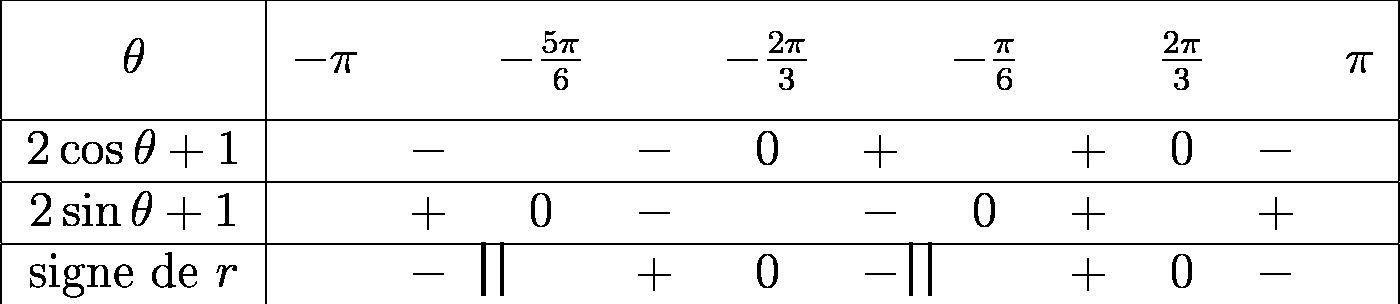
\includegraphics{../images/img005531-1}$$


\textbf{Variations de $r$.} La fonction $r$ est dérivable sur  $[-\pi,\pi]\setminus\left\{-\frac{5\pi}{6},-\frac{\pi}{6}\right\}$ et pour $\theta\in[-\pi,\pi]\setminus\left\{-\frac{5\pi}{6},-\frac{\pi}{6}\right\}$

\begin{center}
$r'(\theta)=\frac{-2\sin\theta(2\sin\theta+1)-2\cos\theta(2\cos\theta+1)}{(2\sin\theta+1)^2}=\frac{-4-2\cos\theta-2\sin\theta}{(2\sin\theta+1)^2}=\frac{-4-2\sqrt{2}\cos\left(\theta-\frac{\pi}{4}\right)}{(2\sin\theta+1)^2}<0$.
\end{center}
La fonction $r$ est strictement décroissante sur $\left[-\pi,-\frac{5\pi}{6}\right[$, sur $\left]-\frac{5\pi}{6},-\frac{\pi}{6}\right[$ et sur $\left]-\frac{\pi}{6},\pi\right]$.
\textbf{Etude quand $\theta$ tend vers $-\frac{5\pi}{6}$.} $\displaystyle\lim_{\substack{\theta\rightarrow-\frac{5\pi}{6}\\ x<-\frac{5\pi}{6}}}r(\theta)=-\infty$ et $\displaystyle\lim_{\substack{\theta\rightarrow-\frac{5\pi}{6}\\ x>-\frac{5\pi}{6}}}r(\theta)=+\infty$. Donc la courbe $\mathcal{C}$ admet une direction asymptotique d'angle polaire $-\frac{5\pi}{6}$ ou encore d'équation $y=\frac{1}{\sqrt{3}}x$. Etudions maintenant l'existence d'une éventuelle droite asymptote et pour cela étudions $\lim_{\theta \rightarrow -\frac{5\pi}{6}}r(\theta)\sin\left(\theta+\frac{5\pi}{6}\right)$.
On pose $h=\theta+\frac{5\pi}{6}$ ou encore $\theta=-\frac{5\pi}{6}+h$ de sorte que $\theta$ tend vers $-\frac{5\pi}{6}$ si et seulement si $h$ tend vers $0$. Quand $h$ tend vers $0$
\begin{align*}\ensuremath
r(\theta)\sin\left(\theta+\frac{5\pi}{6}\right)&=\frac{2\cos\left(-\frac{5\pi}{6}+h\right)+1}{2\sin\left(-\frac{5\pi}{6}+h\right)+1}\sin h=\frac{(1-\sqrt{3}\cos h)+\sin h}{-\sqrt{3}\sin h+(1-\cos h)}\sin h\sim\frac{1-\sqrt{3}}{-\sqrt{3}h}\times h=1-\frac{1}{\sqrt{3}}.
\end{align*}
Par suite, $\mathcal{C}$ admet une droite asymptote $(D_1)$ quand $\theta$ tend vers $-\frac{5\pi}{6}$. De plus

\begin{center}
$M(x,y)\in(D_1)\Leftrightarrow \overrightarrow{OM}.\overrightarrow{v}_{-\frac{5\pi}{6}}=1-\frac{1}{\sqrt{3}}\Leftrightarrow\frac{1}{2}x-\frac{\sqrt{3}}{2}y=1-\frac{1}{\sqrt{3}}\Leftrightarrow y=\frac{1}{\sqrt{3}}x+\frac{2}{3}-\frac{2}{\sqrt{3}}$
\end{center}
\textbf{Etude quand $\theta$ tend vers $-\frac{\pi}{6}$.} $\displaystyle\lim_{\substack{\theta\rightarrow-\frac{\pi}{6}\\ x<-\frac{\pi}{6}}}r(\theta)=-\infty$ et $\displaystyle\lim_{\substack{\theta\rightarrow-\frac{\pi}{6}\\ x>-\frac{\pi}{6}}}r(\theta)=+\infty$. Donc la courbe $\mathcal{C}$ admet une direction asymptotique d'angle polaire $-\frac{\pi}{6}$ ou encore d'équation $y=-\frac{1}{\sqrt{3}}x$.
On pose ensuite $h=\theta+\frac{\pi}{6}$. Quand $h$ tend vers $0$
\begin{align*}\ensuremath
r(\theta)\sin\left(\theta+\frac{\pi}{6}\right)&=\frac{2\cos\left(-\frac{\pi}{6}+h\right)+1}{2\sin\left(-\frac{\pi}{6}+h\right)+1}\sin h=\frac{(1+\sqrt{3}\cos h)+\sin h}{\sqrt{3}\sin h+(1-\cos h)}\sin h\sim\frac{1+\sqrt{3}}{\sqrt{3}h}\times h=1+\frac{1}{\sqrt{3}}.
\end{align*}
Par suite, $\mathcal{C}$ admet une droite asymptote $(D_2)$ quand $\theta$ tend vers $-\frac{\pi}{6}$. De plus

\begin{center}
$M(x,y)\in(D_2)\Leftrightarrow \overrightarrow{OM}.\overrightarrow{v}_{-\frac{\pi}{6}}=1+\frac{1}{\sqrt{3}}\Leftrightarrow\frac{1}{2}x+\frac{\sqrt{3}}{2}y=1+\frac{1}{\sqrt{3}}\Leftrightarrow y=-\frac{1}{\sqrt{3}}x+\frac{2}{3}+\frac{2}{\sqrt{3}}$
\end{center}

\textbf{Tableau de variation de $r$.}


$$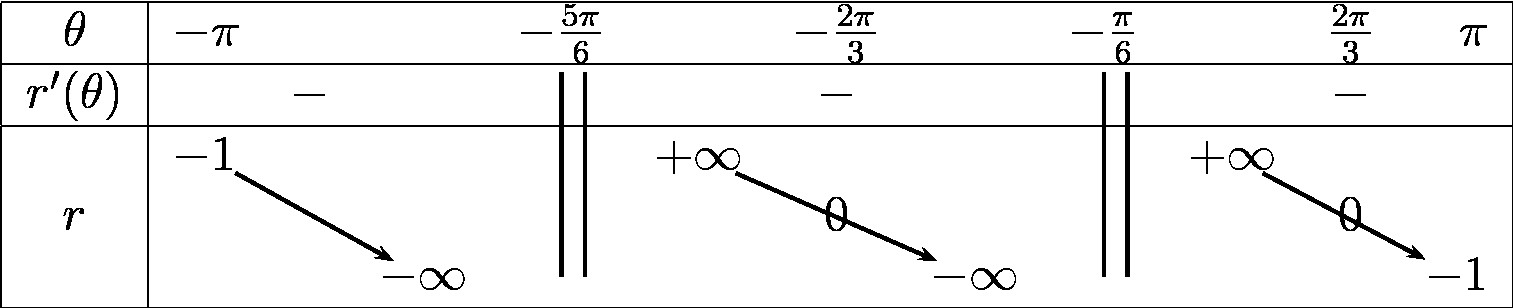
\includegraphics{../images/img005531-2}$$


\textbf{Recherche des points multiples.} Soit $(\theta_1,\theta_2)\in\left([-\pi,\pi]\setminus\left\{-\frac{5\pi}{6},-\frac{\pi}{6}\right\}\right)^2$ tel que $\theta_1<\theta_2$. On suppose de plus que $\theta_1\notin\left\{\pm\frac{2\pi}{3}\right\}$ et $\theta_1\notin\left\{\pm\frac{2\pi}{3}\right\}$ de sorte que $M(\theta_1)\neq O$ et $M(\theta_2)\neq O$. 

\begin{align*}\ensuremath
M(\theta_1)=M(\theta_2)&\Leftrightarrow(\exists k\in\Zz/\;\theta_2=\theta_1+2k\pi\;\text{et}\;r(\theta_2)=r(\theta_1))\;\text{ou}\;(\exists k\in\Zz/\;\theta_2=\theta_1+\pi+2k\pi\;\text{et}\;r(\theta_2)=-r(\theta_1))\\
 &\Leftrightarrow\theta_1\in[-\pi,0],\;\theta_2=\theta_1+\pi\;\text{et}\;r(\theta_2)=-r(\theta_1)\\
 &\Leftrightarrow\theta_1\in[-\pi,0],\;\theta_2=\theta_1+\pi\;\text{et}\;\frac{-2\cos(\theta_1)+1}{-2\sin(\theta_1)+1}=-\frac{2\cos(\theta_1)+1}{2\sin(\theta_1)+1}.
\end{align*}
Maintenant, pour $\theta\in[-\pi,0]\setminus\left\{-\frac{5\pi}{6},-\frac{2\pi}{3},-\frac{\pi}{6}\right\}$

\begin{align*}\ensuremath
\frac{-2\cos(\theta)+1}{-2\sin(\theta)+1}=-\frac{2\cos(\theta)+1}{2\sin(\theta)+1}&\Leftrightarrow-4\cos(\theta)\sin(\theta)+1=4\cos(\theta
)\sin(\theta)-1\Leftrightarrow\sin(2\theta)=\frac{1}{2}\\
 &\Leftrightarrow2\theta\in\frac{\pi}{6}+2\pi\Zz\;\text{ou}\;2\theta\in\frac{5\pi}{6}+2\pi\Zz\Leftrightarrow\theta\in\frac{\pi}{12}+\pi\Zz\;\text{ou}\;\theta\in\frac{5\pi}{12}+\pi\Zz\\
 &\Leftrightarrow\theta\in\left\{-\frac{11\pi}{12},-\frac{7\pi}{12}\right\}.
\end{align*}
Ainsi, les points doubles distincts de l'origine sont $M\left(-\frac{11\pi}{12}\right)=M\left(\frac{\pi}{12}\right)$ et $M\left(-\frac{7\pi}{12}\right)=M\left(\frac{5\pi}{12}\right)$. Sinon, $M\left(-\frac{2\pi}{3}\right)=M\left(\frac{2\pi}{3}\right)=O$.

$$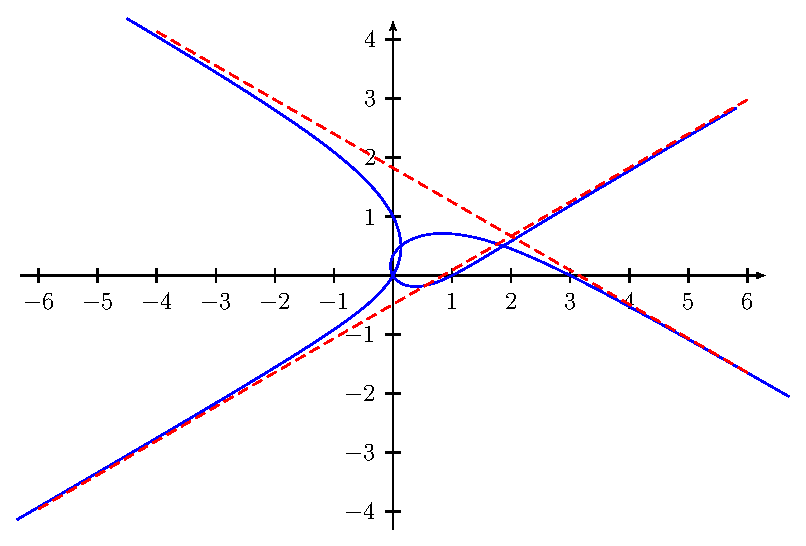
\includegraphics{../images/img005531-3}$$
}
}
